\documentclass[12pt,a4paper]{article}


\usepackage[brazil]{babel}
\usepackage{enumerate}
\usepackage{amsmath}
\usepackage{amssymb}
\usepackage{xspace}
\usepackage{float}
\usepackage{multirow}
\usepackage{bbding}
\usepackage{lipsum}
\usepackage{graphicx}
\usepackage{pgf,tikz,pgfplots}
\pgfplotsset{compat=1.15}
\usepackage{mathrsfs}
\usetikzlibrary{arrows}
\pagestyle{empty}
\usepackage{setspace}
\usepackage{xcolor}
\usepackage{geometry}
\usepackage[T1]{fontenc}
\usepackage{fancyvrb}


\usetikzlibrary{arrows}

\pagestyle{empty}
\pgfplotsset{compat=1.15}

\newtheorem{lema}{\bf Lema}[section]
\newtheorem{teorema}[lema]{\bf Teorema}
\newtheorem{exemplo}[lema]{\bf Exemplo}
\newtheorem{definição}[lema]{\bf Definição}
\newtheorem{proposição}[lema]{\bf Proposição}
\newtheorem{observação}[lema]{\bf Observação}
\newtheorem{corolário}[lema]{\bf Corolário}
\newenvironment{demonstração}{\noindent {\bf Demonstra\c{c}\~{a}o:}}{\hfill${\blacksquare}\hspace*{-2.8mm}{\sqcup} $ \newline}
\newcommand{\Dem}{{\bf Demonstração}\quad}
\newcommand{\cqd}{{\hfill $\rule{2.0mm}{2.0mm}$}\vspace{0.1cm}}


\geometry{a4paper, left=2cm, right=2cm, top=2cm, bottom=2cm}

\begin{document}
	
\begin{figure}[htb]
	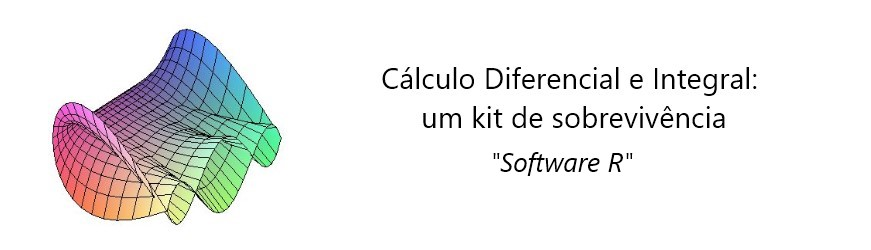
\includegraphics[scale=0.6]{logo.jpg}
\end{figure}

	
	
	\begin{center}Lucas Stefano Xavier de Sousa \\ Orientador: Prof. Dr. Rodrigo Martins.\end{center}
	
	
	\vspace{2cm}
	
	\section*{Produto Vetorial}
	
	O produto vetorial de $\vec{u}$ por $\vec{v}$, (denotado por $\vec{u}\wedge\vec{v}$ ou $\vec{u}\times\vec{v} $) é um vetor, no qual possui as seguintes propriedades:\\
	
	\begin{center}
		\vspace{0.2cm}
		\begin{tabular}{|c|}
			\hline
			\textit{\textbf{Propriedades:}} \\
			1) Se $(\vec{u}, \vec{v})$ é linearmente dependente, então $\vec{u}\wedge\vec{v}=\vec{0}$;\\
			2) Se $(\vec{u}, \vec{v})$ é linearmente independente e $\theta$ é a medida angular entre $\vec{u}$ e $\vec{v}$, então:\\
			
			2.1) $||\vec{u}\wedge\vec{v}|| = ||\vec{u}|| ||\vec{v}|| sen\theta $; \\
			2.2)$\vec{u}\wedge\vec{v}$ é ortogonal a $\vec{u}$ e $\vec{v}$;\\
			
			2.3)$(\vec{u}, \vec{v}, \vec{u}\wedge\vec{v} )$ é uma base positiva.	\\
			\hline
		\end{tabular}
	\end{center}
	
	
	O produto vetorial possui algumas propriedades algébricas, tais como:
	
	\begin{center}
		\vspace{0.2cm}
		\begin{tabular}{|c|}
			\hline
			\textit{\textbf{Propriedades Algébricas:}} \\
			1)$\vec{u}\wedge\vec{v} = - \vec{u}\wedge\vec{v} $;\\
			2)$\vec{u}\wedge(\lambda\vec{u})\wedge\vec{v} = \lambda(\vec{u}\wedge\vec{v})$;\\
			3)$\vec{u}\wedge(\vec{v} + \vec{w}) = \vec{u}\wedge\vec{v} + \vec{u}\wedge{w}$\\
			\hline
		\end{tabular}
	\end{center}
	
	Tem-se que para quaisquer vetores $\vec{u},\vec{v}$ e $\vec{w}$, as igualdades:\\
	
	\begin{center}
		\begin{tabular}{|c|}
			\hline
			\textit{\textbf{Igualdades:}} \\
			1)$(\vec{u}\wedge\vec{v})\wedge\vec{w} = -(\vec{v}\bullet\vec{w})\vec{u}$;\\
			2)$\vec{u}\wedge(\vec{v}\wedge\vec{w})\vec{v} = - (\vec{u}\bullet\vec{}v)\vec{w}$.\\
			\hline
		\end{tabular}
	\end{center}
	
	\section*{Produto Vetorial no R:}
	
	Para facilitar, você pode copiar as áreas em azul e verde, colar no R e substituir as
	verdes pelas informações que você tem, como a função, o ponto, o intervalo etc.\\
	\newline
	$\bullet$ Para calcular o \textbf{produto vetorial} devemos:
	
    	
    {
    	
    	\begin{Verbatim}[commandchars=\\\{\}]
    		
\textcolor{blue}{> install.packages(RSEIS)} #instalar o pacote RSEIS.
\textcolor{blue}{> library(RSEIS)}          #carregar a biblioteca.
\textcolor{blue}{> xprod}\textcolor{green}{(u,v)}              #função que calcula o produto vetorial.
    	\end{Verbatim}
    }
 
	\subsection*{Exemplo 1:}
	
	Considere a base ortonormal positiva B = $(\vec{i}, \vec{j}, \vec{k})$, são dados $\vec{u} = (1,2,3)$ e $\vec{v} = (-1,1,2). $
	\\
	\\	
	Com o auxílio da linguagem R, obtemos:
	
	\begin{verbatim}
		> library(RSEIS)
		> vetoru <- c(1,2,3)
		> vetorv <- c(-1, 1, 2)
		# Utilizando o comando xprod, calculamos o produto vetorial:
		> xprod(vetoru,vetorv)
		[1]  1 -5  3
	\end{verbatim}
	Portanto, tem-se que o produto vetorial de $\vec{u}$ e $\vec{v}$ é o vetor (1,-5,3).\\
	
	
	\bibliographystyle{apalike}
	\begin{thebibliography}{100}
		
		\bibitem {boulos} BOULOS, Paulo; CAMARGO, Ivan. Geometria Analítica-Um tratamento vetorial. São Paulo: Ed. 2005.
		\bibitem{steinbruch} STEINBRUCH, Alfredo; WINTERLE, Paulo. Geometria analítica. McGraw-Hill, 1987.
	\end{thebibliography}
	
\end{document} 